\documentclass[11pt]{article}
\input{\string~/.macros}
\usepackage[a4paper, total={7in, 9in}]{geometry}
\usepackage{bbm}
\usepackage{mathrsfs} % really cursive alphabets
\usepackage{graphicx}
    \graphicspath{{./assets}}
\usepackage{hyperref}
    \hypersetup{colorlinks=true, linktoc=all, linkcolor=blue, citecolor=red}
\usepackage[backend=bibtex,sorting=none]{biblatex}
\usepackage[margin=0cm]{caption}

% random variables
\newcommand\ry{\ensuremath{\mathsf{y}}}
\newcommand\rx{\ensuremath{\mathsf{x}}}
\newcommand\rb{\ensuremath{\mathsf{b}}} 
\newcommand\rc{\ensuremath{\mathsf{c}}}
\newcommand\rz{\ensuremath{\mathsf{z}}}
\newcommand\ru{\ensuremath{\mathsf{u}}}
\newcommand\rw{\ensuremath{\mathsf{w}}}
\newcommand\rpa{\ensuremath{\mathsf{pa}}}
\newcommand\rU{\ensuremath{\mathsf{U}}}
\newcommand\rbx{\ensuremath{\mathsf{\mathbf{x}}}}
\newcommand\rby{\ensuremath{\mathsf{\mathbf{y}}}}
\newcommand\rbu{\ensuremath{\mathsf{\mathbf{u}}}}

\newcommand\bbP{\ensuremath{\mathbbm{P}}}
\newcommand\bbQ{\ensuremath{\mathbbm{Q}}}


% boldsymbols
\renewcommand\bmu{\ensuremath{\boldsymbol{\mu}}}
\newcommand\bSigma{\ensuremath{\boldsymbol{\Sigma}}}
\newcommand\bgamma{\ensuremath{\boldsymbol{\gamma}}}
\newcommand\bomega{\ensuremath{\boldsymbol{\omega}}}
\newcommand\bnu{\ensuremath{\boldsymbol{\nu}}}


% optimization, classes of functions
\newcommand\scrF{\ensuremath{\mathscr{F}}}
\newcommand\scrS{\ensuremath{\mathscr{S}}}
\newcommand\scrP{\ensuremath{\mathscr{P}}}

% independence
\newcommand{\dperp}{\ensuremath{\perp\!\!\!\perp}}
\newcommand{\ndperp}{\ensuremath{\not\!\perp\!\!\!\perp}}

% operators
\newcommand{\prox}{\ensuremath{\mathsf{prox}}}
\addbibresource{optimal_transport}
\addbibresource{registration}


\begin{document}

\section{Diffeomorphic Registration}

\cite{begComputingLargeDeformation2005} proposes lddmm for registering images. The goal of the paper is to register two images $I_0,I_1: \Omega\to\R^d$ where $\Omega\subset\R^n$ (n=2 for 2d images) by computing a diffeomorphic coordinate transformation $\varphi:\Omega\to\Omega$ such that the pullback of $I_0$ by $\varphi^{01}$, i.e. $\varphi.I_0 = I\circ \varphi^{-1}$, is registered to the target image $I_1$. Previous work on non-rigid registration approximates $\varphi$ as locally linear, e.g. $\varphi(x) = x + u(x)$ for some displacement vector field $u:\Omega\to\R^n$; However, this assumption breaks down when there is large displacement of objects within the two images. Instead of solving for the transformation directly, the paper proposes to solve for a time-varying velocity vector field $v_t: \Omega\to\R^n$ for $t\in [0,1]$ that dictates dynamics of time-varying transformations $\phi_t: \Omega\to\Omega$, $\frac{d}{dt} \phi_t = v_t(\phi_t) \quad \phi_0 = \text{Id}$ and that the desired transformation $\varphi$ is the endpoint of the above ODE problem, $\varphi  = \phi_1 = \phi_0 + \int_0^1 v_t(\phi_t) \, dt$.
It has been shown that if the velocity vectors are sufficiently smooth, then $\varphi$ is a diffeomorphic map. Let $V$ be the space of velocity fields with norm $\norm{f}_V = \norm{Lf}_{L^2}$ for $L = (-\alpha \nabla^2 + \gamma)^{\beta} I$, we are interested to find velocity fields that are smooth and that the resulting pullback image is similar to the target image, captured by the follwing energy functional.
\begin{align}
    E(v)
        = \int_0^1 \norm{v_t}_V^2 \, dt + \frac{1}{\sigma^2} \norm{ I_0 \circ \phi_1^{-1} - I_1 }_{L^2}^2
\end{align}
where $v := \pc{v_t}$ satisfies $\dot{\phi_t} =  v_t(\phi_t)$. The velocity fields $v_t$ can be optimized using gradient descent. Once an estimate of velocity field is estimated $\hat{v}$, the resulting transformation $\hat{\varphi}$ can be computed via numerical integration of the ODE system. Of particular interest to this method is that the optimization can be interpreted as finding the (discretized) geodesic path on manifold of diffeomorphisms connecting $I_0,I_1$, and that the length of geodesic $\int_0^1 \norm{v_t}_V \, dt$ is a metric distance between images connected via the diffeomorphism at the end point of the flow.



\section{Geodesic Shooting}

\cite{millerGeodesicShootingComputational2006,vialardDiffeomorphic3DImage2012} are good references for geodesic shooting of point set and images, albeit hard to understand. \cite{joshiLandmarkMatchingLarge2000} proposed large deformation registration for landmarks, \cite{vaillantStatisticsDiffeomorphismsTangent2004,allassonniereGeodesicShootingDiffeomorphic2005} proposed to flow shape along its geodesics using initial momentum for registering landmarks and textured mesh respectively; both are more accessible introduction to geodesic shooting for point set. Jean Feydy's phd thesis is also pretty helpful and gives good intuition \cite{feydyGeometricDataAnalysis2020}.

Instead of integrating a time-varying velocity fields to get a diffeomorphic transformation, geodesic shooting evolves the shape from initial momentum. Let $\Omega \subset\R^D$ be ambient space. Let the space of smooth velocity fields $V$ as a rkhs over $\Omega$ characterized by kernel $k:\Omega\times\Omega\to\R^{D\times D}$ satisfying vector-valued reproducing property $\inner{k(x,\cdot)y}{v}_{V} = \inner{v(x)}{y}_{\R^D}$ for all $y\in\R^D, v\in V$. For landmarks, we assume we are trying to seek time-varying velocity field $v_t\in V$ matching template $(x^1,\cdots,x^n)\subset \Omega^N$ and target $(y^1,\cdots,y^n)\subset\Omega^N$ points.
\begin{align}
    \min_{v_t:t\in [0,1]} \,
        &\frac{1}{2} \int_0^1 \norm{v_t}_V^2 \, dt + \frac{1}{2\sigma^2} \sum_{i=1}^N \norm{\varphi(x^i) - y^i}_{\R^{D}}^2 \\
        \text{where}
            &\quad \varphi = \phi_1 = x + \int_0^1 v_t(\phi_t(x)) \, dt \\
            &\quad \frac{d}{dt}\phi_t(x) = v_t(\phi_t(x)) \quad\quad \phi_0 = \text{Id}
\end{align}
For $\int_0^1 \norm{v_t}_V \, dt < \infty$, $\varphi$ is a diffeomorphism. Let $q_t^i = \phi_t(x^i) \in \R^D$ be application of transformation $\phi_t$ to point $x^i$. Denote $q_t = (q_t^1, \cdots, q_t^N) \in \R^{ND}$ as action of $\phi_t$ to a set of points and $K(q_t,q_t) \in \R^{ND\times ND}$ be kernel matrix for velocity vector field at $q_t$ consisting of $N\times N$ blocks of $K(q^i,q^j) \in \R^{D\times D}$. \cite{joshiLandmarkMatchingLarge2000} argues for a Lagrangian view of previous Eulerian problem. Instead of solving for flow velocity $v(x,t)$ for all $x\in\Omega, t\in [0,1]$, it suffices to solve for the flow velocity $\dot{q}_t$ of particles,
\begin{align}
    \min_{\dot{q}_t:t\in [0,1]}
        &\frac{1}{2} \int_0^1 \inner{\dot{q}_t}{K(q_t,q_t)^{-1}\dot{q}_t} \, dt + \frac{1}{2\sigma^2} \norm{q_1 - y}_{\R^{ND}}^2
\end{align}
and that the resulting flow velocity in the Eulerian coordinates $\Omega$ can be interpolated from $\dot{q}_t$,
\begin{align}
    v_t(x)
        = K(x, q_t) p_t
    \quad\quad
    p_t
        = K(q_t, q_t)^{-1} \dot{q}_t
\end{align}
where $p_t^i \in \R^{D}$ is the momenta associated with point $q_t^i$. As a side note, this interpolation is akin to computing posterior mean of a gaussian process regression of velocity fields, i.e. $v_t(x) = K(x,q_t) K(q_t,q_t)^{-1} \dot{q}_t$. Note the integrand of rkhs norm can be viewed as Lagrangian of of a system of ND particles. \cite{millerGeodesicShootingComputational2006} argues the dynamics of these particles in canonical coordinates $(q_t,p_t)$ follows the Geodesic equations with initial condition $q_0 = x, p_0$,
\begin{align}
    \dot{q}_t
        = \frac{\partial \sH(q_t,p_t)}{\partial p}
    \quad\quad
    \dot{p}_t
        = - \frac{\partial \sH(q_t,p_t)}{\partial q}
    \label{eq:geodesic_equations}
\end{align}
and that the Hamiltonian $\sH(q_t,p_t) = \frac{1}{2}\inner{p_t}{K(q_t,q_t)p_t} = \frac{1}{2}\inner{K(q_t,q_t)^{-1}\dot{q}_t}{\dot{q}_t}$ is preseved by the flow, $\sH(q_0,p_0)  = \sH(q_t,p_t)$ for all $t\in [0,1]$ and therefore, $\int_0^1 \sH(q_t,p_t) \, dt = \sH(q_0, p_0) = \frac{1}{2} \inner{ p_0 }{ K(q_0,q_0) p_0 }$. We arrive at a registration problem where we optimize over the initial or \textit{shooting momentum} $p_0$ so that $q_1 := q_1(x,p_0)$ is close in some sense to target $y$,
\begin{align}
    \min_{p_0\in\R^{ND}} \,
        \frac{1}{2} \inner{ p_0 }{ K(x,x) p_0 } + \frac{1}{2\sigma^2} \norm{q_1 - y}_{\R^{ND}}^2
    \label{eq:optimization_momentum_landmark}
\end{align}
Optimization involves a forward integration of $(q_t,p_t)$ via (\ref{eq:geodesic_equations}) to get transformed particles $q_1$, compute the gradient of objective (\ref{eq:optimization_momentum_landmark}) with respect to initial momentum, and do gradient update iteratively.


\begin{center} 
\begin{figure}[h!]
    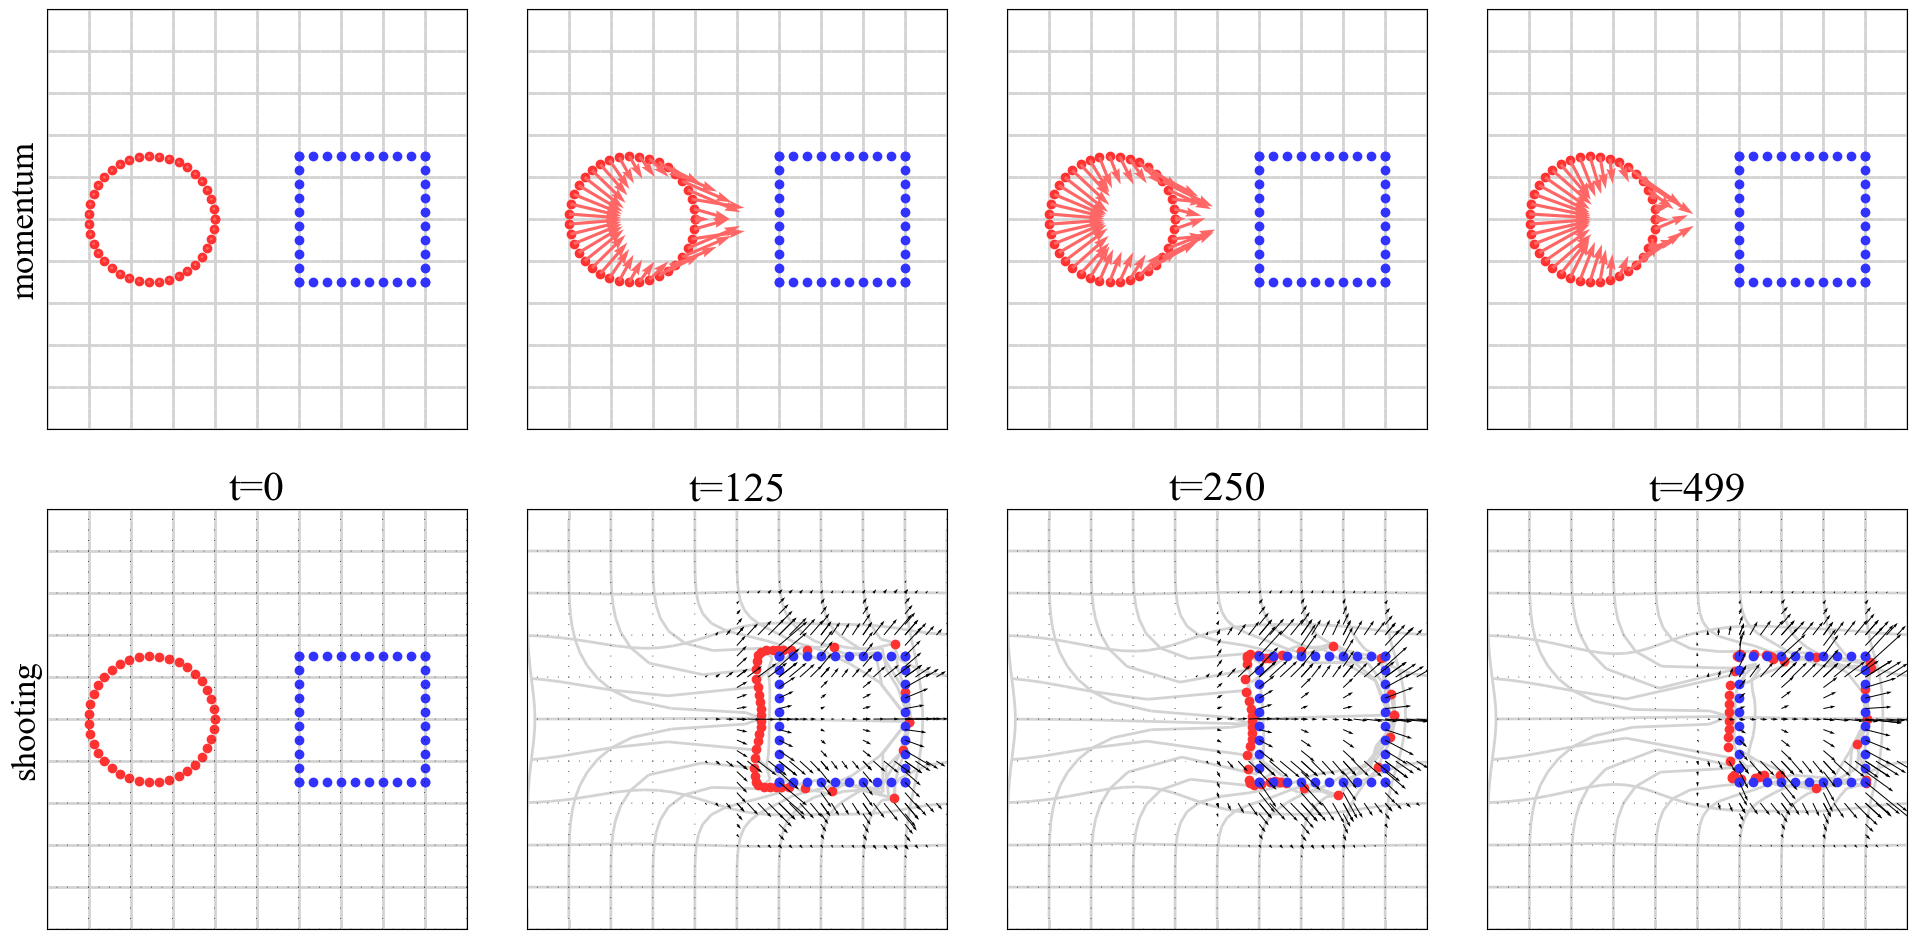
\includegraphics[width=\textwidth]{assets/plt_shooting} 
    \caption{Geodesic shooting with an Euler integrator with time step of $\delta t = .1$. The velocity field is represented using a radial basis kernel with $\sigma=.25$. We show trajectory of $q_t$ (red dots) with momentum $p_t$ (blue arrow) and interpolated velocity fields at grid points (black). We see Hamiltonian is approximately conserved!}
    \label{fig:plt_shooting}
\end{figure} 
\end{center} 


\begin{center} 
\begin{figure}[h!]
    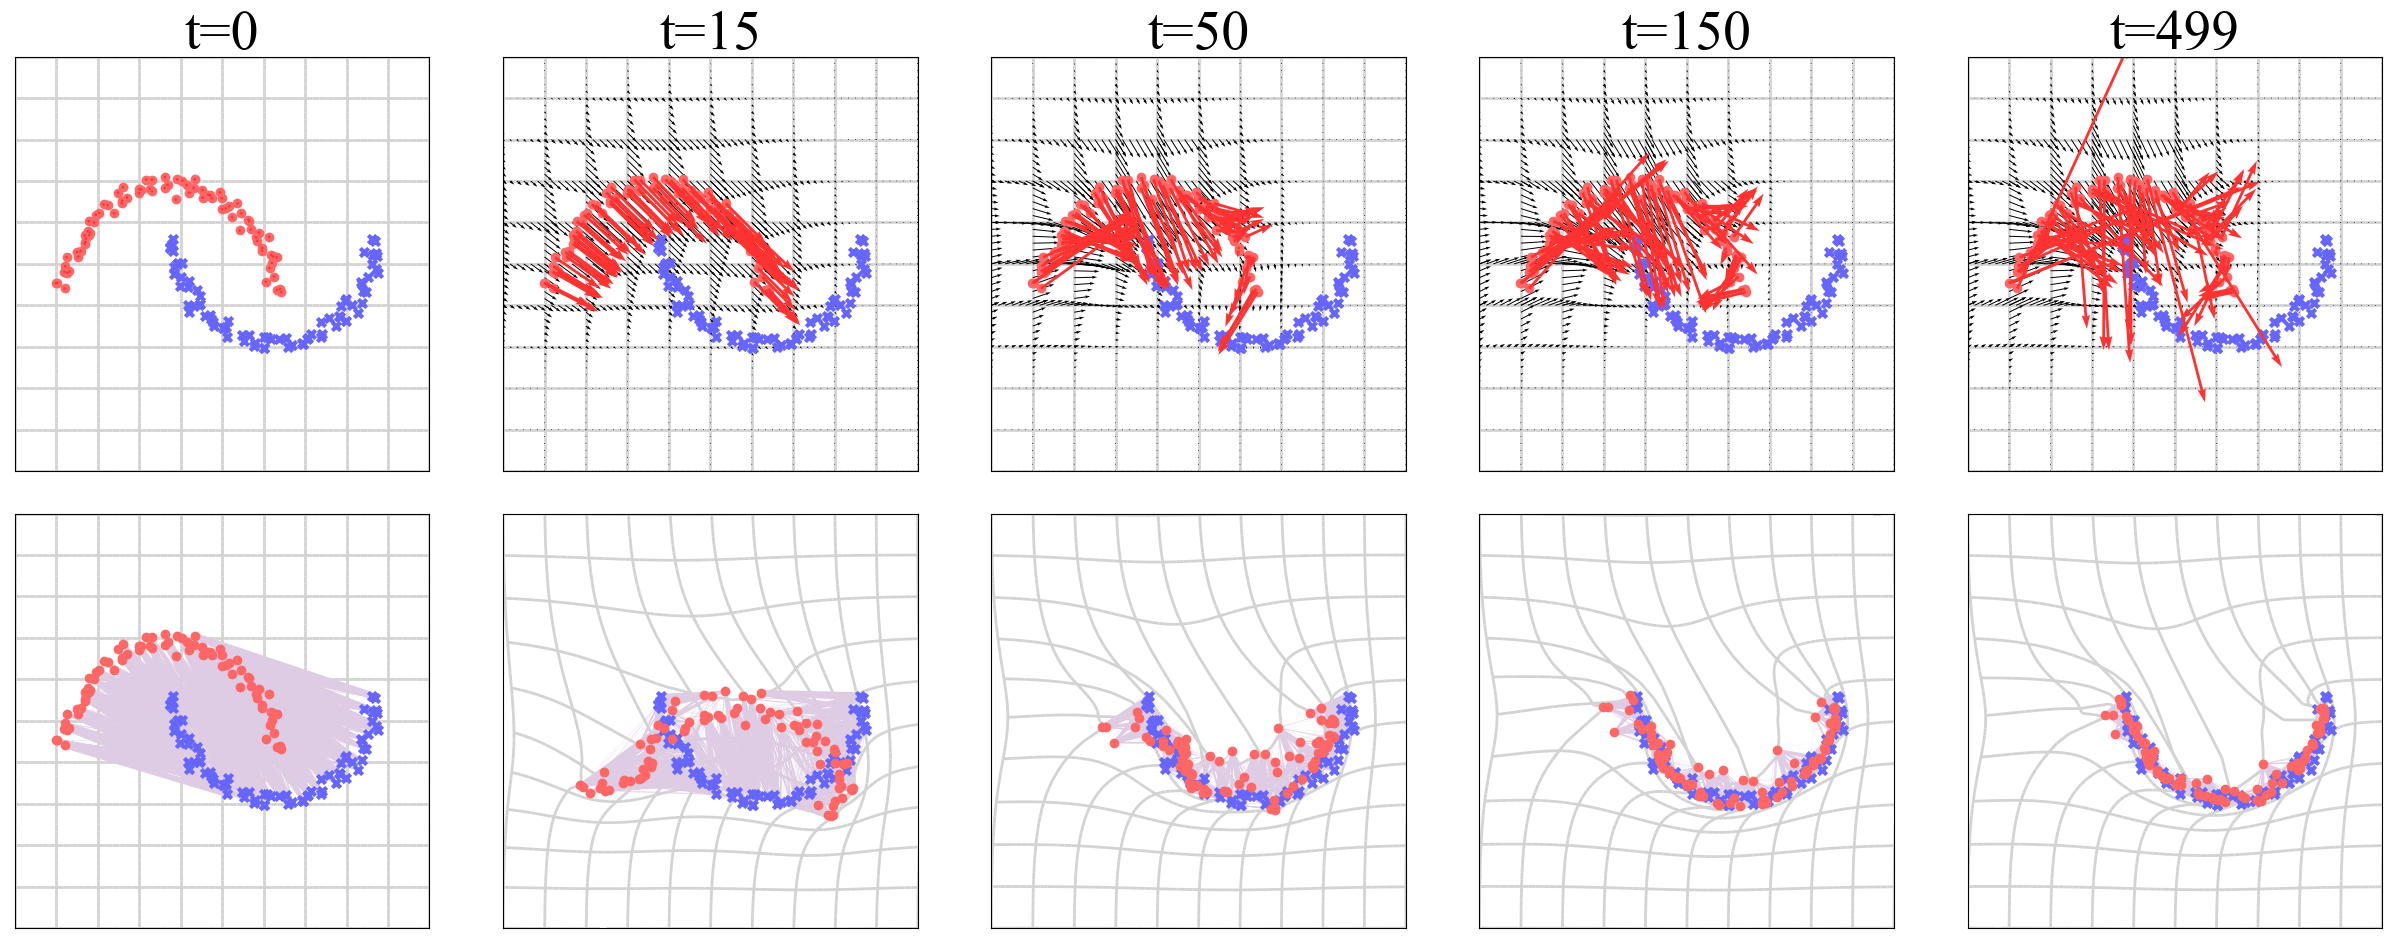
\includegraphics[width=\textwidth]{assets/plt_lddmm_points_moons_training}
    \caption{Training dynamics of usage of optimal transport cost for registering points}
    \label{fig:plt_lddmm_points_training}
\end{figure}
\end{center} 


 
\begin{center} 
\begin{figure}[h!]
    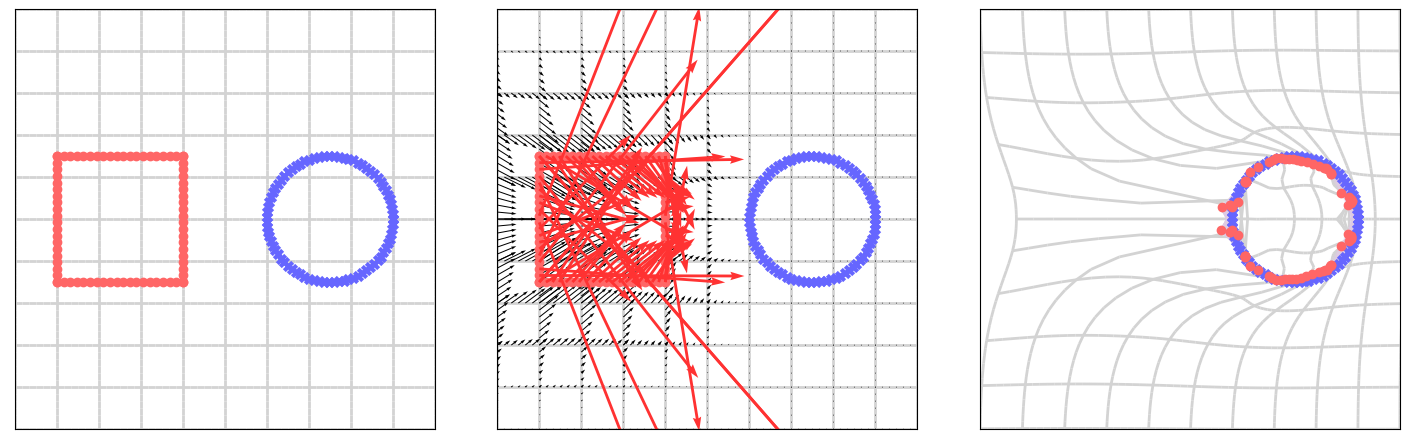
\includegraphics[width=\textwidth]{assets/plt_lddmm_points_shapes} 
    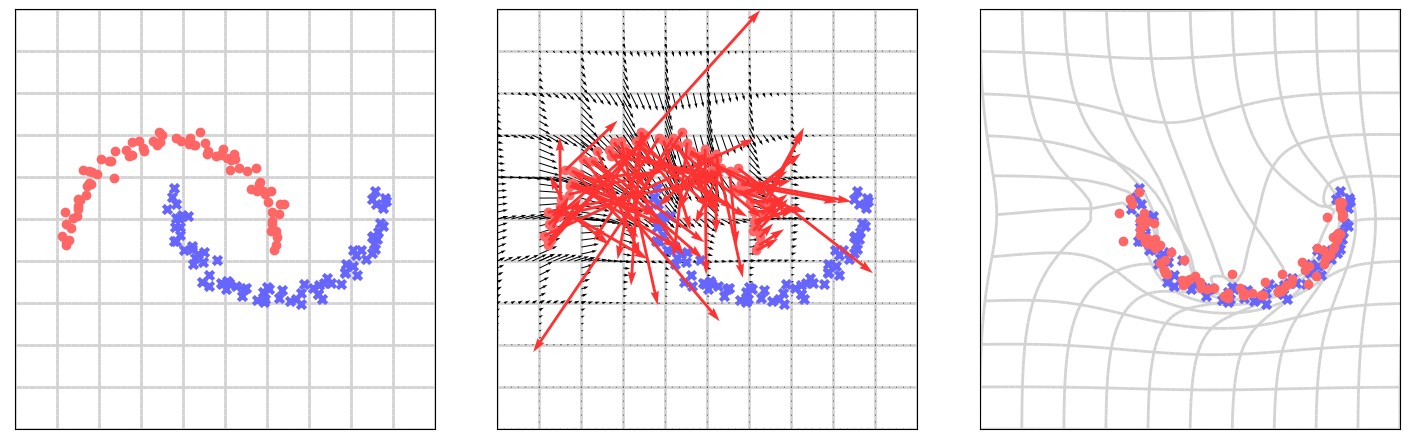
\includegraphics[width=\textwidth]{assets/plt_lddmm_points_moons} 
    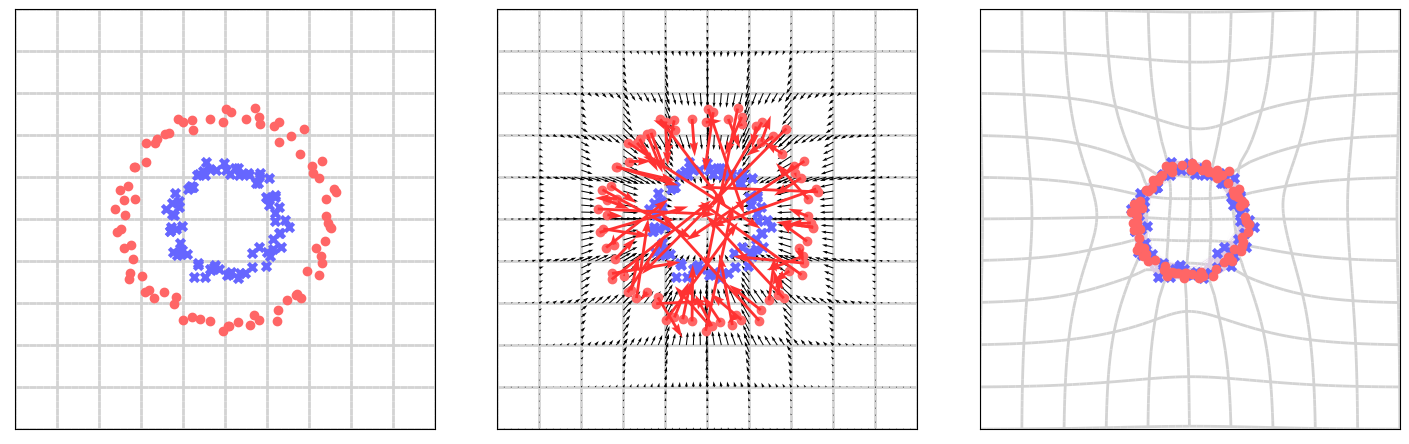
\includegraphics[width=\textwidth]{assets/plt_lddmm_points_circles} 
    \caption{lddmm with geodesic shooting and entropic regularized unbalanced optimal transport distance as matching loss. Points are encoded as sum of deltas with uniform weights. Shooting's kernel is a sum of radial basis kernel with $\ell \in \pc{.025,.15,.3}$ so as to be able to distinguish points both close and far away. }
    \label{fig:plt_lddmm_points}
\end{figure}
\end{center} 
    
  



\newpage
\printbibliography 




\end{document}
